\documentclass[a4paper, 11pt]{article}
\usepackage{graphicx}
\usepackage{amsmath}
\usepackage[pdftex]{hyperref}
\usepackage{epstopdf}
\usepackage{multirow}
\usepackage[table,xcdraw]{xcolor}

% Lengths and indenting
\setlength{\textwidth}{16.5cm}
\setlength{\marginparwidth}{1.5cm}
\setlength{\parindent}{0cm}
\setlength{\parskip}{0.15cm}
\setlength{\textheight}{22cm}
\setlength{\oddsidemargin}{0cm}
\setlength{\evensidemargin}{\oddsidemargin}
\setlength{\topmargin}{0cm}
\setlength{\headheight}{0cm}
\setlength{\headsep}{0cm}

\renewcommand{\familydefault}{\sfdefault}

\title{Data Mining: Learning from Large Data Sets - Fall Semester 2015}
\author{caifa.zhou@geod.baug.ethz.ch\\ pungast@student.ethz.ch\\ llara@student.ethz.ch\\}
\date{\today}

\begin{document}
\maketitle

\section*{Explore-Exploit tradeoffs in Recommender Systems} 

To learn the policy of exploring and exploiting choices, and to then give recommendations for news articles to the user, we implemented a LinUCB algorithm with a hybrid linear model.

\textbf{Summary:} we used the LinUCB algorithm to solve the exploration vs. exploitation problem, which is formulated in the multi-armed bandit framework. The idea of the hybrid model is to combine different recommendation techniques, here the content-based and collaborative filtering. In the model $\delta$ is set to 0.3 and $\alpha = 1 + \sqrt{ln(2/\delta)/2}$ 

The functions \textbf{recommend, update} and \textbf{set\_articles} in the policy file are completed as follows.  

First, in the \textbf{set\_articles} function all the necessary parameters are initialized, including the identity matrix M, her inverse, the zero vector b, the zero matrix B and the weights w and a list of article IDs is created.

The \textbf{recommend} function returns the optimal matching article $x_{t}$ for the user: 
$x_{t} = \underset{x\in A_{t}}{\operatorname{argmax}}~\mathrm{UCB_{x}}$ with $\mathrm{UCB_{x}} = \mathrm{\hat{w}_{x}^{T}z_{t} + \alpha \sqrt{z_{t}^{T}M_{x}^{-1}z_{t}}}$ by using the LinUCB algorithm. 

Last, with the \textbf{update} function, the model is updated according to the LinUCB hybrid model given that the recommendation was successful, i.e. the user clicked on the proposed article. 
 

\pagebreak


\section*{Extracting Representative Elements} 

To extract 100 clusters of representative elements from a large dataset, we used k-means ++ and k-means in the mapper and reducer, where the mapper outputs 500 points (cluster centers) for each batch and the reducer finds the final 100 based on the output of the mappers.

The \textbf{mapper} is constructed as follows. Data is processed in batches of 10000 data points.

The cluster centers of each stream are initialised using k-means++ to find a solution in reasonable time, and then sequential k-means is run. Weights are assigned to all points, whereby points farther away from the existing centers get a higher weight and thus have a higher probability to be selected. Iteratively the subsequent centers are chosen from the remaining data points with probability proportional to its squared distance ($\left \| x_{i} - \mu_{j} \right \|^{2}_{2}$) from the closest existing cluster center $\mu_{j}$.

Third, the sequential k-means algorithm is implemented to compute representative elements ($\mu_{j}$) one at a time. The centers (means) are given by the vector $\mu$ with $\mu_{1},...,\mu_{k}$, the algorithm calculates $\partial L/\partial \mu$ with $ \partial L(x,\mu) = min \left \| x_{i} - \mu_{j} \right \|^{2}_{2}$. If $\mu_{i}$ is closest to x,  $\mu_{i}$ is replaced by $$frac{1}{k_{i}}\sum_{j=1}^{k_{i}}{x_{j}}$$where $k_i$ is the number of data points assigned to $i^{th}$ cluster. 
Last, the emit function prints the centers into stdout.

The \textbf{reducer} receives the cluster centers from all mappers. As in the mapper, the reducer finds runs k-means++ in this reduced space to find initial cluster centers. Sequential k-means algorithm is then run on these initial centers to find the final representative elements. \pagebreak

\section*{Large Scale Image Classification} 
To classify the images into the categories nature and people, using a Support Vector Machine as classifier and Parallel Stochastic Gradient Descent procedure, a Map and Reduce function was implemented. 

\textbf{Summary:} we used a primal version of the Support Vector Machine (implemented in sklearn.svm.LinearSVC) and transformed the original features into Random Fourier Features.

The \textbf{mapper} is constructed as follows. First, it reads each line, extracts the features and transforms those. Then it adds the transformed features to the batch and calculates the weight vector on that batch, processes the batch and starts a new one until all input is processed. If the batch size is infinite, each mapper treats its whole input as a single batch.

The particular parameters used in the best submission were: infinite batch size and 800 random features.

A batch of examples is processed by first calculating the weight vectors, with $\eta = \frac{1}{\sqrt{t +1}}$, such that if $y\mathrm{w^{T}x} < 1$ then update the weights, such that $\mathrm{w'_{t}} \leftarrow\mathrm{w + \eta _{t}}y \mathrm{x}$ and set $\mathrm{w_{t+1}} = \mathrm{min \left \{1,\frac{1/\sqrt{\lambda }}{\left \| w'_{t} \right \|} \right \}}$.

As the last step of the processing of one batch, the emit function prints the weight vector from the batch into standard output.

The \textbf{reducer} receives the weight vectors from the mapper. A weight vector is thereby represented by one input line, which is parsed into a vector. Then the reducer calculates the average of all the vectors received from mappers and prints the space-separated coefficients of the model.

The groupwork was done as following. First we sat together and discussed the assignment and overall structure of the project. Taivo Pungas created a first draft of the mapper and reducer, Caifa Zhou continuously contributed to the structure of the mapper and both tested different versions. Lara Lingelbach wrote the report. \pagebreak

\section*{Approximate near-duplicate search using Locality Sensitive Hashing} 

To detect duplicate videos a locality sensitive hashing solution using MapReduce was implemented.
Below, our solution is described in steps.

The \textbf{mapper} reads each line of input, extracts the video ID and shingles, deletes recurring elements in the shingles and sorts the shingles. It then calculates the signature matrix column for each video, partitions it into bands, hashes each band and emits the result.

To calculate the signature matrix columns, we create n hash functions of the form $h_{a,b}(x) = ax + b \bmod N$ (where $N=20001$) by generating parameter vectors $a$ and $b$ of size n containing random nonnegative integers. Using the MinHash approach and each generated $h_{a,b}$, we calculate the column of the signature matrix corresponding to the current video.

To generate candidate pairs, we partition the signature matrix column into $b$ bands and hash each band with a linear hash function (resulting in a bucket ID). The mapper then emits a key-value pair where the key is a string concatentation (band ID + bucket ID) and the value is a tuple (signature matrix column, video ID). In the \textbf{reducer}, all videos that have the same key are then compared pairwise to find out whether the videos were actually similar (with bitwise similarity $\geq 0.9$ in the signature columns of the two videos).

Each machine uses the same seed when generating random numbers for the hash functions.

Given the constraint $ br \leq 1024 $, the parameters $b$ and $r$ were chosen to empirically produce the highest F1-score on the training set, resulting in $(b, r)=(20, 50)$.

The general workflow of the mapper and reducer are illustrated in Figure~\ref{fig: Digraph}. 

\begin{figure}[!htb]
\centering
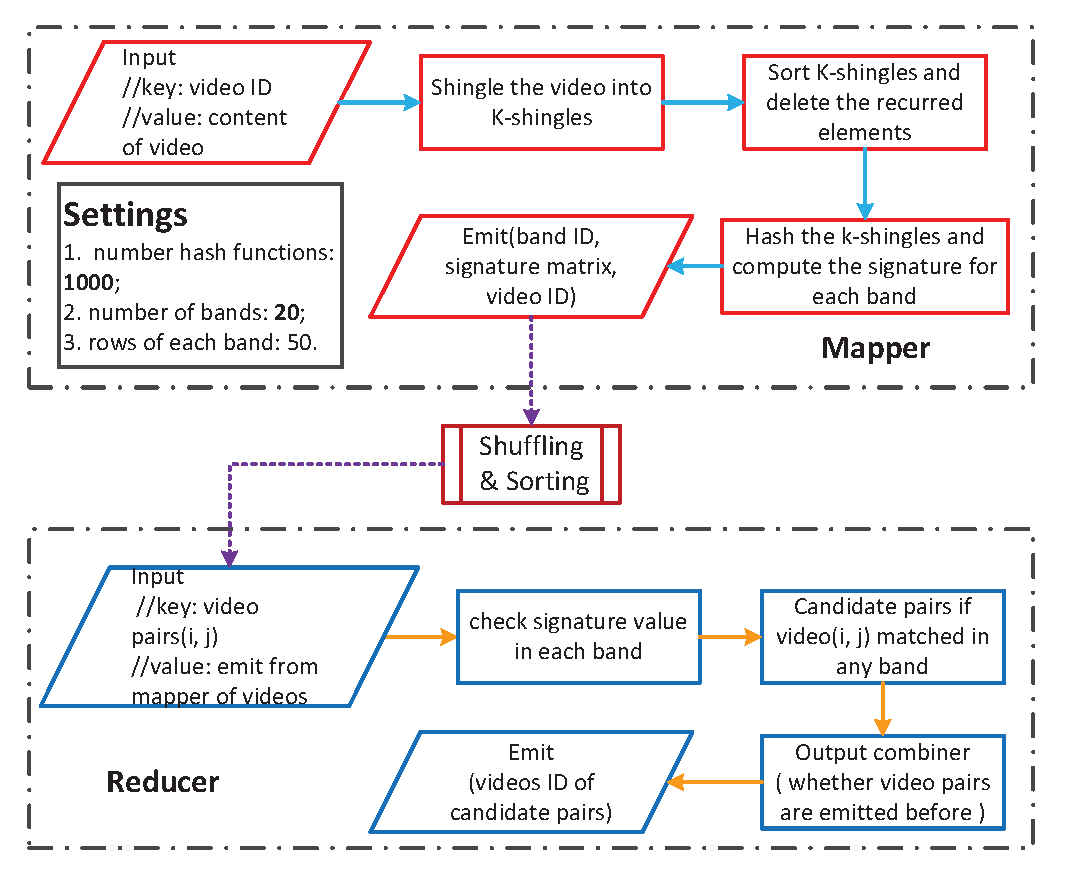
\includegraphics[scale=.7]{workflow_project_1.eps}
\caption{Workflow of the locality sensitive hashing solution using MapReduce.}
\label{fig: Digraph}
\end{figure}

The groupwork was done according to each member's background. First we sat together and discussed the assignment and overall structure, then Caifa Zhou implemented the mapper, Taivo Pungas created the reducer as well as revised the mapper and Lara Lingelbach generated the report. 


\end{document} 
